% !TEX root = ./main.tex


%-----------------------------------------------------------------------------
%    STARTER
%-----------------------------------------------------------------------------

\documentclass{backend/backend}
\usepackage{backend/font}
\usepackage{backend/colors}
\usepackage{backend/structure}
\usepackage{backend/informations}

%-----------------------------------------------------------------------------
%    PRESENTATION SLIDES
%-----------------------------------------------------------------------------

\begin{document}


\begin{frame}
    \titlepage
\end{frame}

\section*{Introduction}
\showtoctrue % active l'affichage des slides de transition

\begin{frame}{Introduction}
    
    \begin{block}{1999 : Howgrave-Graham et Smart }
        latAtk
    \end{block}

    2001 : Publication dans le journal \textit{Designs, Codes and Cryptography}
    
\end{frame}

\begin{frame}{Introduction}
    
   +++
\end{frame}

\begin{frame}{Sommaire}

        \small
        \tableofcontents

\end{frame}



\section{Préambule} % ordre historique
\subsection{Réseaux Euclidiens}

\begin{frame}{Réseaux Euclidiens}
    
    
    Un réseau $L$ est un sous-groupe discret de $\mathbb{R}^n$.\\
    
    Cette structure peut être décrite par une base $\mathcal{B}$ de $d$ vecteurs indépendants \{$b_1, \dots b_d$\}.
    
    
    En posant $A$ la matrice dont les lignes sont les $d$ vecteurs de $\mathcal{B}$, on peut écrire :
    $$L = \{\mathbf{x}A : \mathbf{x} \in \mathbb{Z}^n\}$$
\end{frame}



\begin{frame}{Closest Vector Problem}

\begin{columns}

    \begin{column}{0.5 \linewidth}
        \begin{itemize}
            \item Pour un vecteur $\mathbf{t}$ de $\mathbb{R}^n$, trouver le vecteur de $L$ le plus proche.
            \item NP-Difficile
        \end{itemize}
    \end{column}

\end{columns}
\end{frame}


\begin{frame}{Réduction de base}

+++
    
\end{frame}


\begin{frame}{Algorithme de réduction de réseau}
    \begin{figure}
        \centering
        \caption{Comparaison du facteur d'approximation et le temps de calcul entre LLL, BKZ et Sieving AlicePelletMary}
        \label{fig:algoReduc}
    \end{figure}
\end{frame}


\begin{frame}{Approximation du CVP}

    \Large{ \textbf{Babaï}} \normalsize :\\
    
    $$ \gamma = 2\left(\frac{2}{\sqrt{3}}\right)^d $$

    avec $d$ le rang du réseau.\smallbreak

    Algorithme du plan proche de Babai :
    \begin{enumerate}
        \item une base \(\mathcal{B} \in \mathbb{Z}^{d \times n}\)
        \item un vecteur cible \(t \in \mathbb{Z}^n\)
    \end{enumerate}
    Une réduction de réseau avant de projeter itérativement \(t\) sur chaque vecteur de base réduit successif. La projection arrondie est ensuite soustraite de \(t\) pour obtenir un nouveau vecteur plus proche du point du réseau.
    
\end{frame}


\subsection{Signature DSA}


\begin{frame}{Digital Signature Algorithm}

    La sécurité de la signature DSA, repose sur le problème du logarithme discret dans le groupe $({Z} / p \mathbb{Z})^{\times}$ avec $p$ premier et suffisamment grand.\smallbreak

    Paramètres publics:
    \begin{enumerate}
        \item $p_{1024}$ et $q_{160}$, deux nombres premiers et tel que $q |(p-1)$, dsaFIPS
        \item $g$ un générateur de $({Z} / p \mathbb{Z})^{\times}$
     \end{enumerate}
     \smallbreak
     Clé secrète : $x  \leftarrow \mathbb{Z} / q \mathbb{Z}$ \smallbreak
     Clé publique : $h=g^{x}$

    \begin{center}
        $(p,q,g,h)$
    \end{center}

\end{frame}

\begin{frame}{Protocole de signature}

    $f$ une fonction de hachage : SHA-1 \smallbreak    
    
    Soit $m \in \mathbb{Z} / q \mathbb{Z}$ , $y  \overset{\$}{\leftarrow} \mathbb{Z} / q \mathbb{Z}$ \smallbreak
    
    \begin{empheq}[box={\equations}]{equation}
       b \equiv (m + x f\left(g^{y}\right))y^{-1} \quad(\bmod q) \label{eq:signature}
    \end{empheq}

    \begin{center}
        $(g^y, b)$
    \end{center}

    Pour vérifier la signature :
    \begin{empheq}[box={\equations}]{equation*}
       g^{m} \times h^{f(g^{y})}=(g^{y})^b
    \end{empheq}
\end{frame}

% \begin{frame}{Interêt des courbes elliptiques}
%     \begin{table}[ht]
%     \centering
%     \caption{Taille de clés pour une sécurité équivalente entre la signature DSA et la signature avec les courbes elliptiques (EC). Issu de guide_elliptic_crypto, p.19}
%     \begin{tabular}{|lccccc|}
%         \toprule
%         & \multicolumn{5}{c|}{\textbf{Security level (bits)}} \\
%         & 80 & 112 & 128 & 192 & 256 \\
%         \midrule
%         DSA paramètre $p$  & 1024 & 2048 & 3072 & 8192 & 15360 \\
%         EC paramètre $n$ & 160  & 224  & 256  & 384  & 512  \\
%         \bottomrule
%     \end{tabular}
% \end{table}
% \end{frame}

\subsection{Signature ECDSA}
\begin{frame}{Elliptic Curve DSA}

    $E$ une courbe elliptique d'ordre $n$ un nombre premier, soit $P$ un point de $E$ et $f$ notre fonction de hachage. \smallbreak
    
    Clé secrète $x \leftarrow \mathbb{Z}/n\mathbb{Z}$\\ 
    Clé publique $Q = xP$\\

    \begin{empheq}[box={\equations}]{equation*}
       r  \overset{\$}{\leftarrow} \mathbb{Z}/n\mathbb{Z}, rP = (x_R, y_R)
    \end{empheq}
    
    La signature est alors donnée par $\sigma = (\sigma_1, \sigma_2) = (x_R \mod n, s)$, où :
    \begin{empheq}[box={\equations}]{equation}
       s \equiv r^{-1}(x(x_R \mod n) + f(m)) \pmod{n}.
    \end{empheq}

    
\end{frame}

\begin{frame}{Signature ECDSA - vérification}
    
    Vérification de $(\sigma_1, \sigma_2)$ : \\
    \begin{enumerate}
        \item $ u_1 \equiv f(m) \sigma_2^{-1} \pmod{n}$
        \item $ u_2 \equiv \sigma_1 \sigma_2^{-1} \pmod{n}$
    \end{enumerate}

    $(x_1, y_1) = u_1 P + u_2 Q$
    \begin{empheq}[box={\equations}]{equation}
       \sigma_1 \equiv x_1
    \end{empheq}


\end{frame}

\section{Traces \& Préparation}


\begin{frame}{Illustration d'une trace}
    
    Appelons $x$ la valeur dont on veut récupérer les bits d'informations, admettons par exemple que $x$ s'écrit ainsi :
    
    \begin{center}
    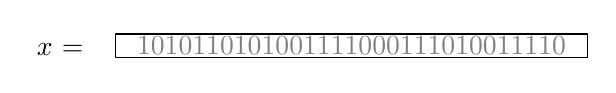
\begin{tikzpicture}
        \draw (0,0) rectangle (6,0.3) ;
        \draw (-0.7,0.1) node {$x$ =};
        \draw (3,0.15) node[gray] {1010110101001111000111010011110};
    
    \end{tikzpicture}
    \end{center}
    
    L'information inconnue de $x$, en rouge sur les schémas ci-dessous, peut être organisée de différentes manières. La plus simple étant le cas contigu où juste un bloc de bits est manquant :\smallbreak
    
    
    \begin{enumerate}
      \item[Cas contigu :]
        \begin{center}
            %left
            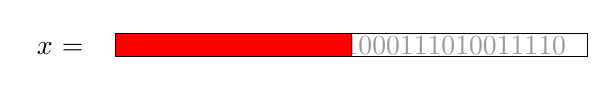
\begin{tikzpicture}
                \draw (0,0) rectangle (6,0.3);
                \draw (-0.7,0.1) node {$x$ =};
                \draw (3,0.14) node[gray!80] {1010110101001111000111010011110};
                \filldraw[fill=red] (0,0) rectangle (3,0.3);
            \end{tikzpicture}
            \smallbreak
    
            %right
            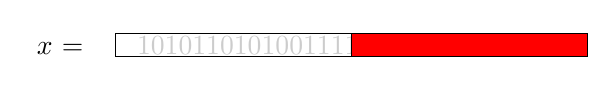
\begin{tikzpicture}
                \draw (0,0) rectangle (6,0.3);
                \draw (-0.7,0.1) node {$x$ =};
                \draw (3,0.14) node[gray!40] {1010110101001111000111010011110};
                \filldraw[fill=red] (3,0) rectangle (6,0.3);
            \end{tikzpicture}
            \smallbreak
    
            %center
            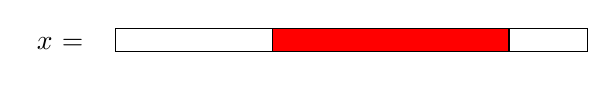
\begin{tikzpicture}
                \draw (0,0) rectangle (6,0.3);
                \draw (-0.7,0.1) node {$x$ =};
                \filldraw[fill=red] (2,0) rectangle (5,0.3);
            \end{tikzpicture}
            \smallbreak
       \end{center}
    \end{enumerate}
\end{frame}

\begin{frame}{Illustration d'une trace - cas non contigu}
 
    Mais nous prenons aussi en compte le cas où l'information manquante est séparée en plusieurs blocs :
    
    \begin{enumerate}
       \item[Cas non-contigu :]
       \begin{center}
            %non contigous
            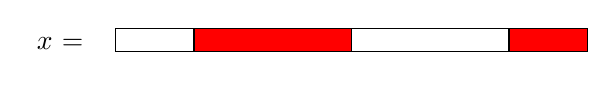
\begin{tikzpicture}
                \draw (0,0) rectangle (6,0.3);
                \draw (-0.7,0.1) node {$x$ =};
                \filldraw[fill=red] (1,0) rectangle (3,0.3);
                \filldraw[fill=red] (5,0) rectangle (6,0.3);
            \end{tikzpicture}
            \smallbreak
    
            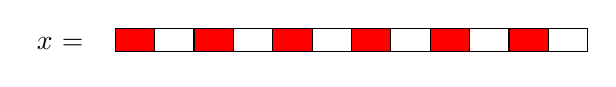
\begin{tikzpicture}
                \draw (0,0) rectangle (6,0.3);
                \draw (-0.7,0.1) node {$x$ =};
                \foreach \k in {0.5, 1.5, ..., 6}
                    {\filldraw[fill=red] (\k - 0.5,0) rectangle (\k,0.3);}
    
            \end{tikzpicture}
            \smallbreak
            
            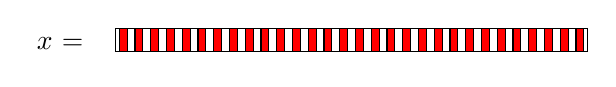
\begin{tikzpicture}
                \draw (0,0) rectangle (6,0.3);
                \draw (-0.7,0.1) node {$x$ =};
                \foreach \k in {0.15, 0.35, ..., 6.05}
                    {\filldraw[fill=red] (\k - 0.1,0) rectangle (\k,0.3);}
            \end{tikzpicture}
        \end{center}
    \end{enumerate}
    
    \bigskip
    
\end{frame}



\section{Attaque}

\subsection{Mise en équations}

\begin{frame}{Signatures et équations}

    Attaque par canal auxiliaire => bits d'information sur les clés éphémères $y_i$
    
    Objectif : retrouver entièrement une clé éphémère et d'en déduire la clé privée $x$
    
    On récupère $h$ signatures => $h$ équations pour $1\leq i \leq h$:
    
    \begin{empheq}[box={\equations}]{equation}
       m_{i} - b_{i} y_{i} + x f\left(g^{y_{i}}\right) \equiv 0\quad(\bmod q)
    \end{empheq}
    \smallbreak
    
    On peut ensuite réarranger nos équations, avec $A$ et $B$ entiers, sous cette forme $y_{i} + x A_{i} + B_{i} \equiv 0\quad(\bmod  q)$.
    Pivot de Gauss pour exprimer $x$ en fonction de $y_h$ :
    \begin{empheq}[box={\equations}]{equation}
       y_{i} + y_{h} \times A^{\prime}_{i} + B^{\prime}_{i} \equiv 0 \quad(\bmod q)\label{eq:milieu}
    \end{empheq}

\end{frame}

\begin{frame}{Simplification des équations}

    \begin{empheq}[box={\equations}]{equation}
    y_{i}=\alpha_{i}^{\prime}+2^{\lambda_{i}} z_{i}+2^{\mu_{i}} \alpha_{i}^{\prime \prime}\label{eq:cle_y}
    \end{empheq}

    \begin{center}
    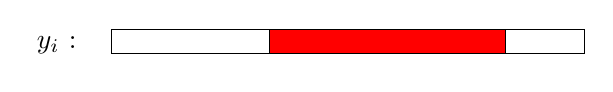
\begin{tikzpicture}
        \draw (0,0) rectangle (6,0.3);
        \draw (-0.7,0.1) node {$y_i$ :};
        \filldraw[fill=red] (2,0) rectangle (5,0.3);
    \end{tikzpicture}
    \end{center}

    
    On connaît les $\alpha_{i}^{\prime}$, $\alpha_{i}^{\prime \prime}$, $\lambda_{i}$ et $\mu_{i}$. Nos inconnues sont les $z_{i}$ et on définit $X_i$ leurs bornes supérieures  :
    
    $$
    0 \leq z_{i}<X_{i}=2^{\mu_{i}-\lambda_{i}}
    $$
    
    On simplifie une dernière fois nos équations pour obtenir :
    \begin{empheq}[box={\equations}]{equation}
      z_{i}+s_{i} z_{h}+t_{i} = 0 \quad(\bmod q)  
    \end{empheq}

\end{frame}




\subsection{Construction de réseau}
\begin{frame}{Réseau et CVP}
    \vspace*{-0.28cm}
    
    $$
    A=\left(\begin{array}{ccccc}
    -1 & s_{1} & s_{2} & \ldots & s_{n} \\
    0 & q & 0 & \cdots & 0 \\
    0 & 0 & q & & 0 \\
    \vdots & & & \ddots & \vdots \\
    0 & \cdots & \cdots & \cdots & q
    \end{array}\right) \in M_{(n+1),(n+1)}(\mathbb{Z})
    $$
    
    Réseau $L=\left\{\mathbf{x} A: \mathbf{x} \in \mathbb{Z}^{n+1}\right\}$ issu de $A$. 
    Un vecteur $\mathbf{v}$ de $L$ s'exprime ainsi :
    $$
    \mathbf{v} = (-x_0 ,\, x_0s_1 + x_1q, \, \ldots, \, x_0s_n +x_nq)\in \mathbb{Z}^{n+1}
    $$
    
    \begin{empheq}[box={\equations}]{equation*}
       z_i \equiv -z_hs_i - t_i \quad(\bmod q) 
    \end{empheq}
 
\end{frame}



\begin{frame}
    \begin{empheq}[box={\equations}]{equation*}
       z_i \equiv -z_hs_i - t_i \quad(\bmod q) 
    \end{empheq} 
    En prenant :
    
    $$
    \mathbf{t}=\left(0, t_{1}, t_{2}, \ldots, t_{n}\right) \in \mathbb{Z}^{n+1}
    $$
    
    On sait qu'il existe :
    $$
    \mathbf{v} - \mathbf{t} = (z_h,\, z_1,\, \ldots,\, z_n) \in \mathbb{Z}^{n+1}
    $$

    $$
    \Vert \mathbf{v} - \mathbf{t} \Vert^2 \leq \sum_{i=0}^{n} X_i^2
    $$ 
\end{frame}




\begin{frame}{Non-contigu}
    \begin{empheq}[box={\equations}]{equation*}
        y_i = z'_i + \sum_{j=1}^{d}z_{i,j}2^{\lambda_{i,j}}
    \end{empheq}

    \begin{center}
    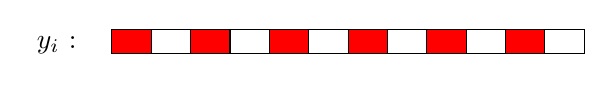
\begin{tikzpicture}
        \draw (0,0) rectangle (6,0.3);
        \draw (-0.7,0.1) node {$y_i$ :};
        \foreach \k in {0.5, 1.5, ..., 6}
            {\filldraw[fill=red] (\k - 0.5,0) rectangle (\k,0.3);}
    \end{tikzpicture}
    \end{center}

Notre système d'équation devient :
    $$
    z_{i, 1}+\sum_{j=2}^{d} s_{i, j} z_{i, j}+\sum_{j=1}^{d} r_{i, j} z_{0, j}+t_{i} \equiv 0 \quad(\bmod q) 
    $$
    
\end{frame}


\begin{frame}
    
$$
A=\left(\begin{array}{c|c}
-I_{d(n+1)-n} & R^{t} \\
& S \\
\hline 0 & -q I_{n}
\end{array}\right) \times D
$$

Où $R=\left(r_{i, j}\right)$ et $S$ correspond à la matrice

$$
S=\left(\begin{array}{ccc}
\mathbf{s}_{1} & & 0 \\
& \ddots & \\
0 & & \mathbf{s}_{n}
\end{array}\right) \in M_{n(d-1), n}(\mathbb{Z})
$$

avec $\mathbf{s}_{i}$ le vecteur colonne $\left(s_{i, j}\right)_{j=2}^{d}$.\smallbreak
    
\end{frame}






\section{Résultats}

\subsection{DSA 1024 160}

\begin{frame}{Comparaison avec l'article}
+++
\end{frame}

\end{document}